\chapter{Hardware Implementation}
\label{Chapter2}

% This chapter details the foundational hardware architecture and the software environment that brings your custom SoC to life. It explains the tools, frameworks, and specific components used in the design and implementation of your system.

\section{Chisel HDL}
\label{sec:chisel_hdl}

\begin{figure}[htbp]
    \centering
    \begin{subfigure}[b]{0.3\textwidth}
        \centering
        
\includegraphics[width=\linewidth]{Images/01_Chisel_chisel.pdf}
    \end{subfigure}%
    \hfill
    \begin{subfigure}[b]{0.2\textwidth}
        \centering
        
\includegraphics[width=\linewidth]{Images/01_Chisel_firrtl.pdf}
    \end{subfigure}%
    \hfill
    \begin{subfigure}[b]{0.2\textwidth}
        \centering
        
\includegraphics[width=\linewidth]{Images/01_Chisel_chips_alliance.pdf}
    \end{subfigure}
    \caption{Logos: Chisel, FIRRTL, and CHIPS Alliance.}
    \label{fig:chisel_ecosystem_logos}
\end{figure}

\subsection{Theoretical Aspects of Chisel}
\label{sec:chisel_theoretical}
Chisel (Constructing Hardware In a Scala Embedded Language) is a hardware construction language (HCL) embedded in the Scala programming language. Unlike traditional Hardware Description Languages (HDLs) like Verilog or VHDL, Chisel leverages the power of a modern software language to describe hardware circuits. This approach allows for more productive and robust hardware design, especially for complex systems \cite{bachrach2012chisel}. Chisel is permissively licensed (Apache 2.0) under the guidance of CHIPS Alliance.

% Motivation for Chisel
The motivation behind Chisel stems from the increasing complexity of SoC designs. Traditional HDLs, while effective for describing hardware at a low level, can become cumbersome and error-prone when dealing with large, highly parameterized, or configurable systems. Chisel aims to address these challenges by introducing software engineering principles like abstraction, parameterization, and generation into the hardware design process. It seeks to improve design reusability, reduce development time, and enhance verification capabilities.

% Key Concepts/Benefits
Key concepts and benefits of Chisel include:
\begin{itemize}
    \item \textbf{Generators:} Chisel excels at creating parameterized hardware generators. Designers can write code that generates specific hardware instances based on a set of parameters. This is extremely powerful for creating configurable components like CPUs, caches, or accelerators, where a single generator can produce many different variations tailored to specific needs.
    \item \textbf{High-Level Abstraction:} By being embedded in Scala, Chisel allows designers to express hardware at a much higher level of abstraction than traditional HDLs. This includes using object-oriented programming, functional programming constructs, and rich type systems to describe complex hardware structures more concisely and intuitively.
    \item \textbf{Modularity \& Composability:} Chisel promotes the creation of modular and composable hardware components. Designs can be broken down into smaller, reusable modules that can be easily interconnected to build larger systems. This aligns with modern software engineering practices and facilitates team-based design.
    \item \textbf{Type Safety:} Scala's strong static type system, inherited by Chisel, helps catch many common design errors at compile time rather than during lengthy simulations. This leads to more robust designs and faster debugging cycles.
    \item \textbf{FIRRTL:} Chisel is powered by FIRRTL (Flexible Intermediate Representation for RTL), a hardware compiler framework implemented by LLVM CIRCT. Chisel designs are compiled into FIRRTL, which serves as a common interchange format that can be transformed and optimized before being converted into Verilog for synthesis or simulation. This decoupling allows for a vibrant ecosystem of tools and backends to operate on Chisel-generated hardware \cite{chipyard}.
\end{itemize}

\begin{figure}[htbp]
    \centering
    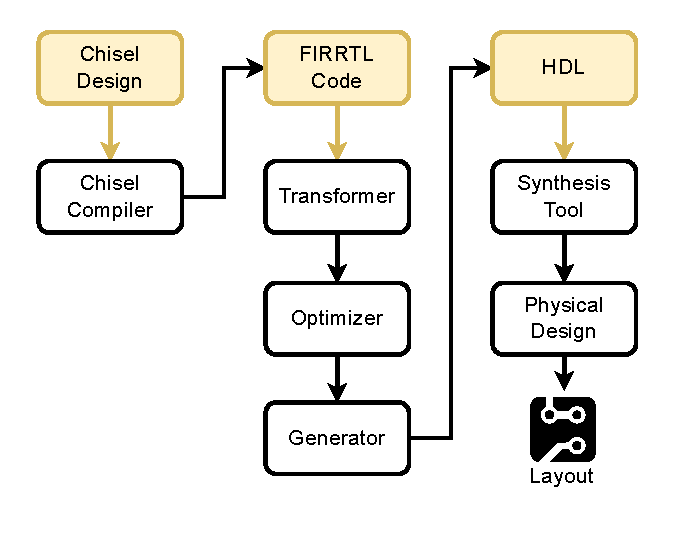
\includegraphics[width=0.75\linewidth]{Images/01_Chisel_flow.pdf}
    \caption{Chisel and FIRRTL workflow.}
    \label{fig:chisel_flow}
\end{figure}

\subsection{Chisel Implementation and Relevance to Project}
\label{sec:chisel_implementation}
% Role in Your Design
In this project, Chisel is the fundamental hardware description language used for defining the core components of the SoC. Specifically, it is the underlying language for the Rocket Chip SoC generator, the Gemmini accelerator, and the overarching Chipyard framework that integrates these elements. While this project did not involve writing extensive custom Chisel code from scratch, understanding Chisel is crucial as it defines the structure and behavior of the pre-existing generators that were configured and integrated.

% Advantages Utilized
The primary advantages of Chisel utilized in this project are its generative capabilities and parameterization. For instance, the Rocket core and Gemmini accelerator are highly parameterized Chisel generators. This allowed for the specific configuration of the CPU (e.g., RV64I, cache sizes) and the Gemmini accelerator (e.g., systolic array dimensions, scratchpad size) to meet the project's requirements without needing to modify low-level RTL. The Chipyard framework leverages these Chisel-based generators to construct the final SoC design.

\section{Chipyard for SoC Design Framework}
\label{sec:chipyard_framework}

\begin{figure}[htbp]
    \centering
    
\includegraphics[width=0.75\linewidth]{Images/02_Chipyard_ChipyardLogo.pdf}
    \caption{Chipyard logo.}
    \label{fig:chipyard_logo}
\end{figure}

\subsection{Theoretical Aspects of Chipyard}
\label{sec:chipyard_theoretical}
Chipyard is an open-source, integrated System-on-Chip (SoC) design framework that promotes agile development methodologies for complex, custom hardware systems \cite{chipyard}. It provides a comprehensive ecosystem that brings together a vast collection of RTL generators, software toolchains, simulation environments, and VLSI implementation flows. The primary goal of Chipyard is to enable rapid architectural exploration, design, validation, and physical implementation of SoCs, particularly those incorporating RISC-V cores, specialized hardware accelerators, and heterogeneous compute elements.

% Core Components
Chipyard's key constituents include:
\begin{itemize}
    \item \textbf{Chisel-based RTL Generators:} At its core, Chipyard relies heavily on Chisel for hardware generation. It integrates a rich library of open-source, generator-based IP blocks, including RISC-V CPU cores (like Rocket, BOOM), cache hierarchies, memory interconnects (e.g., TileLink), peripherals, and domain-specific accelerators like Gemmini. These generators allow for highly parameterized and composable hardware designs.
    \item \textbf{Software Toolchains:} Chipyard provides a complete set of software development tools, including RISC-V cross-compilers (GCC, LLVM), linkers, debuggers (GDB), and tools for building bare-metal applications and full Linux distributions (e.g., using Buildroot or Yocto through FireMarshal). This enables software development to proceed concurrently with hardware design.
    \item \textbf{Simulation Environments:} Chipyard supports multiple simulation methodologies for design verification and performance analysis:
    \begin{itemize}
        \item Software RTL Simulation: Cycle-accurate simulation using open-source tools like Verilator or commercial simulators (e.g., VCS, QuestaSim) for detailed debugging and functional verification \cite[p.~29]{chipyard}.
        \item FPGA-Accelerated Simulation (FireSim): For faster, full-system validation with long-running, complex workloads, Chipyard integrates FireSim. FireSim enables cycle-exact, massively parallel simulation on cloud-hosted FPGAs (e.g., Amazon EC2 F1 instances), providing a scalable and accessible platform for pre-silicon performance evaluation and software testing \cite{karandikar2018firesim, chipyard}.
    \end{itemize}
    \item \textbf{Verification Infrastructure:} The framework incorporates infrastructure for unit testing, integration testing, and full-system verification. This includes testing harnesses, example test suites, and continuous integration (CI) methodologies.
    \item \textbf{VLSI Implementation (Hammer):} For physical design and tapeout, Chipyard includes Hammer, an open-source VLSI flow that abstracts process-technology and EDA-tool specifics. Hammer aims to make physical design scripts more portable and reusable across different manufacturing processes and toolchains \cite{chipyard}.
\end{itemize}

% Design Flow
The typical Chipyard design flow starts with high-level SoC configuration using Scala-based configuration files. These files specify the desired IP blocks, their parameters, and how they are interconnected. Chisel then elaborates this configuration into FIRRTL, which can undergo various transformations. The FIRRTL is then converted to Verilog RTL, which can be used for software simulation, FPGA emulation (e.g., using FireSim or direct FPGA synthesis), or ASIC implementation using Hammer. Concurrently, software workloads, including operating systems like Linux, can be built and run on the simulated or emulated hardware.

\begin{figure}[htbp]
    \centering
    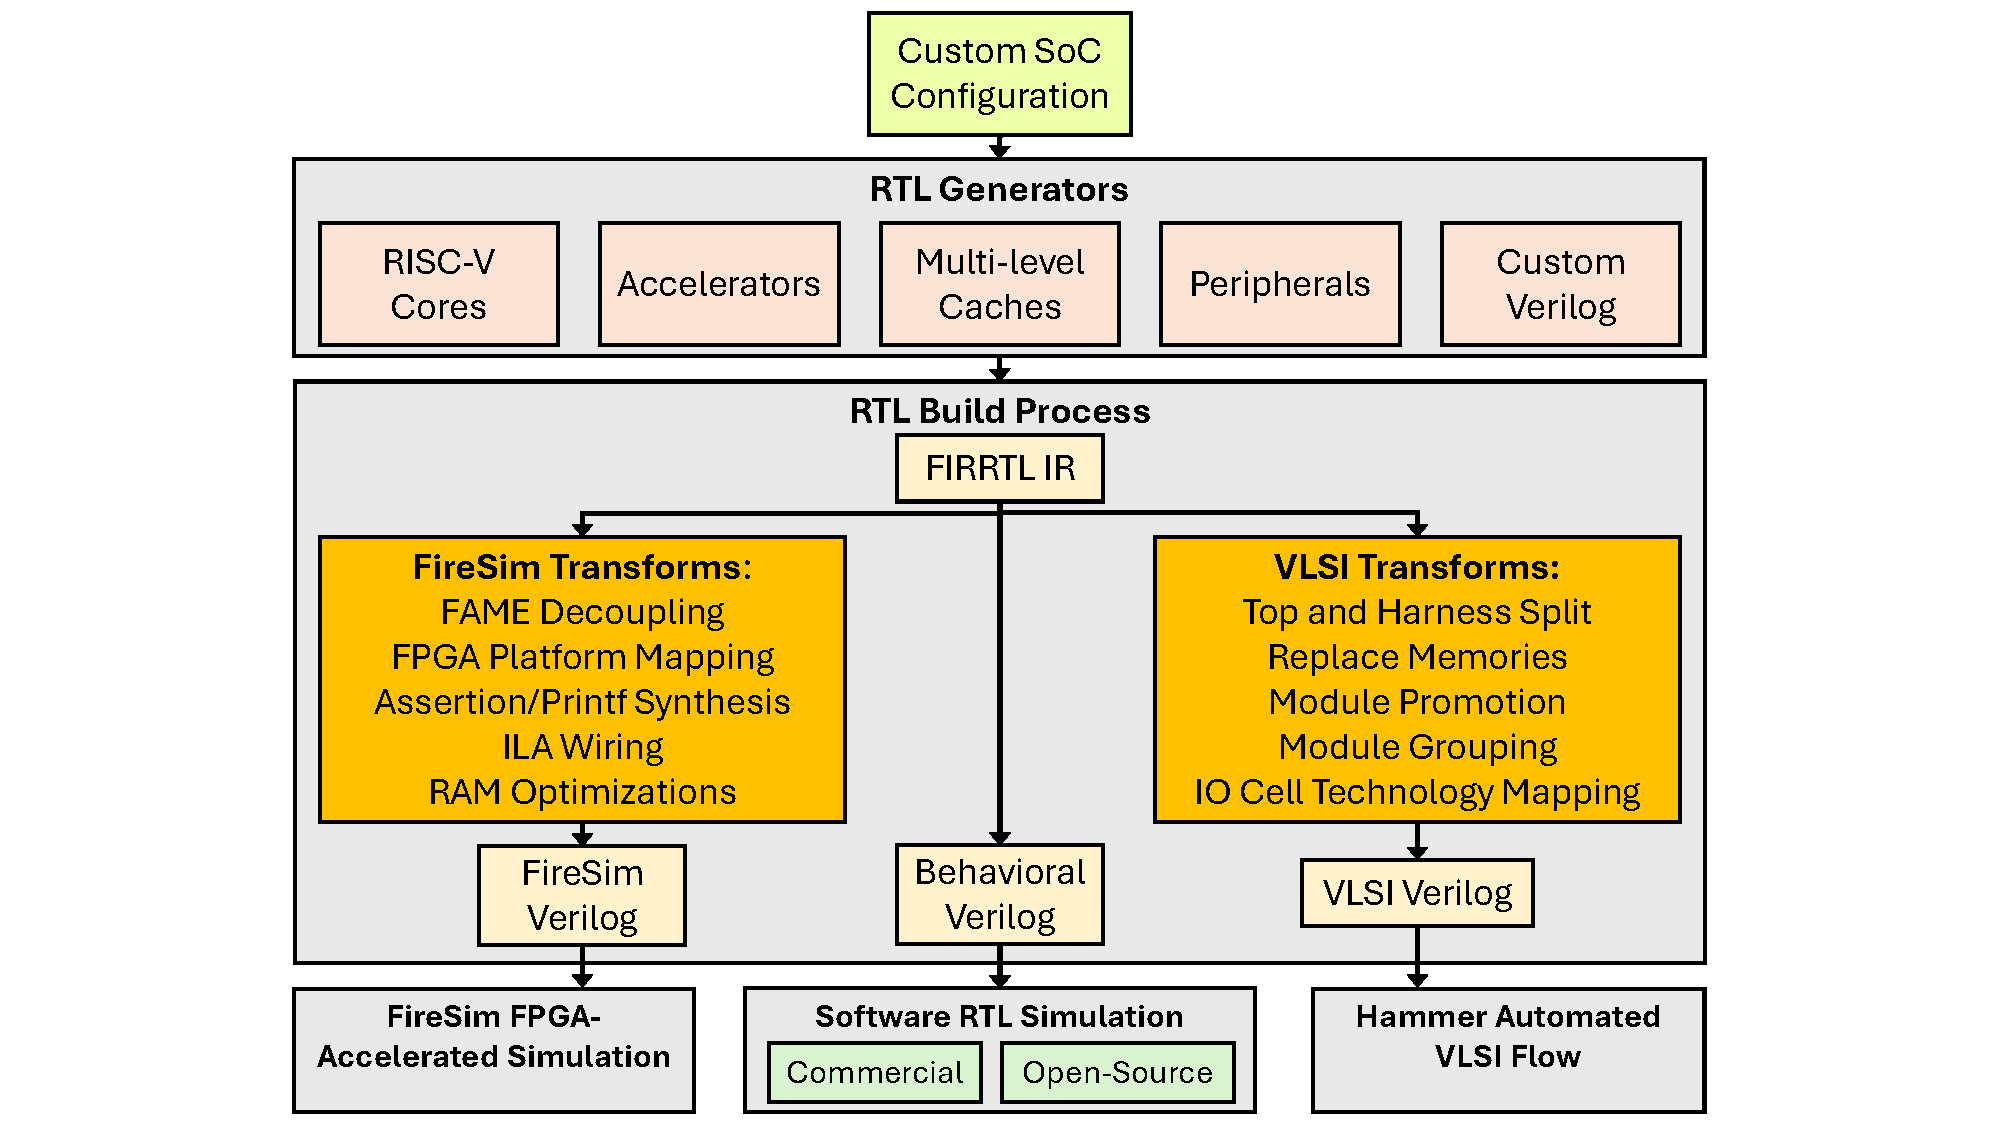
\includegraphics[width=0.75\linewidth]{Images/02_Chipyard_ChipyardFlow.pdf}
    \caption{Multiple disparate design flows supported by the Chipyard framework through generators and transformations. A series of FIRRTL transformations consumes generators with a custom configuration, and outputs appropriate Verilog and associated collateral for different design stage platforms.}
    \label{fig:chipyard_flow}
\end{figure}

\subsection{Chipyard Implementation and Relevance to Project}
\label{sec:chipyard_implementation}
% How You Used Chipyard
In this research, Chipyard served as the foundational framework for generating the custom SoC. The process involved:
\begin{enumerate}
    \item Setting up the Chipyard environment and its dependencies.
    \item Defining a custom SoC configuration that specified the desired Rocket Core variant, Gemmini accelerator parameters, memory system details, and other peripheral components.
    \item Utilizing Chipyard's build system to invoke Chisel and generate the Verilog RTL for the configured SoC.
    \item Employing Chipyard's integrated tools (or tools compatible with its output) for simulation and further downstream processing towards FPGA implementation.
\end{enumerate}
This research utilizes Chipyard as the primary framework for constructing and evaluating the Rocket Chip-based SoC with the Gemmini accelerator. The specific SoC configuration developed is identified as \texttt{Rocket64b1gem16}.

% Your SoC Configuration
Chipyard was used to configure and integrate the specific Rocket Core chosen for this project and the Gemmini accelerator. The \texttt{Rocket64b1gem16} configuration specifies a 64-bit Rocket Core (a "big" core variant suitable for Linux) integrated with a Gemmini unit featuring a 16x16 systolic array. Chipyard's configuration system managed the parameterization of these components and their connection within the SoC fabric, including setting up the TileLink interconnect and memory system interfaces.

\section{RISC-V, Rocket Core, and Rocket Chip}
\label{sec:riscv_rocket}

\subsection{Theoretical Aspects of RISC-V, Rocket Core, and Rocket Chip SoC Generator}
\label{sec:riscv_rocket_theoretical}
% RISC-V ISA
\subsubsection{RISC-V Instruction Set Architecture (ISA)}
RISC-V is an open, free, and extensible instruction set architecture, representing a significant departure from proprietary ISAs \cite{asanovic2014riscv}. Its openness fosters collaboration and innovation in processor design across academia and industry.

% Key Features
Key features of RISC-V include:
\begin{itemize}
    \item \textbf{Modularity:} The ISA is defined by a base integer instruction set (e.g., RV32I, RV64I) and a set of standard, optional extensions (e.g., 'M' for multiplication/division, 'A' for atomics, 'F' for single-precision floating-point, 'D' for double-precision, 'C' for compressed instructions). The combination IMAFD is often denoted by 'G' (general-purpose) \cite{asanovic2016rocketchip}.
    \item \textbf{Extensibility:} RISC-V reserves opcode space for custom user-defined extensions, allowing for tight integration of specialized co-processors and instructions.
    \item \textbf{Privileged Architecture:} It defines multiple privilege levels (Machine, Supervisor, User) and mechanisms for virtual memory (MMU) and interrupt handling, essential for supporting operating systems like Linux \cite{waterman2015riscvpriv}.
\end{itemize}

% Advantages
Advantages of RISC-V include its openness, which eliminates licensing fees and restrictions, its flexibility for customization, and its suitability for a wide range of applications from embedded systems to high-performance computing. This has led to a rapidly growing ecosystem of cores, tools, and software.

\subsubsection{Rocket Core}

\begin{figure}[htbp]
    \centering
    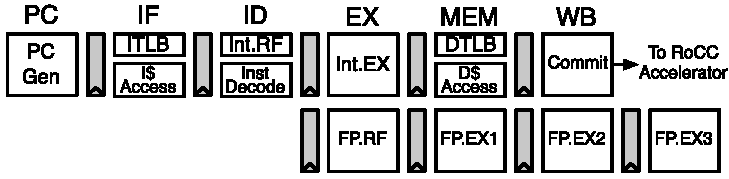
\includegraphics[width=0.75\linewidth]{Images/03_RocketCore_RISCV_Rocket5Pipeline.pdf}
    \caption{The Rocket core pipeline.}
    \label{fig:rocket_core_pipeline}
\end{figure}

Rocket is a 5-stage in-order scalar core generator that implements the RV32G and RV64G ISAs. It has an MMU that supports page-based virtual memory, a non-blocking data cache, and a front-end with branch prediction. Branch prediction is configurable and provided by a branch target buffer (BTB), branch history table (BHT), and a return address stack (RAS). For floating-point, Rocket makes use of Berkeley's Chisel implementations of floating-point units. Rocket also supports the RISC-V machine, supervisor, and user privilege levels. A number of parameters are exposed, including the optional support of some ISA extensions (M, A, F, D), the number of floating-point pipeline stages, and the cache and TLB sizes.
Rocket can also be thought of as a library of processor components. Several modules originally designed for Rocket are re-used by other designs, including the functional units, caches, TLBs, the page table walker, and the privileged architecture implementation (i.e., the control and status register file).

The Rocket Custom Coprocessor Interface (RoCC) facilitates decoupled communication between a Rocket processor and attached coprocessors. Many such coprocessors have been implemented, including crypto units (e.g., SHA3) and vector processing units. The RoCC interface accepts coprocessor commands generated by committed instructions executed by the Rocket core. The commands include the instruction word and the values in up to two integer registers, and commands may write an integer register in response. The RoCC interface also allows the attached coprocessor to share the Rocket core's data cache and page table walker, and provides a facility for the coprocessor to interrupt the core. These mechanisms are sufficient to construct coprocessors that participate in a page-based virtual memory system. Finally, RoCC accelerators may connect to the outer memory system directly over the TileLink interconnect, providing a high-bandwidth but coherent memory port. The Hwacha vector-fetch unit makes use of all of these features and has driven the development of RoCC into a sophisticated coprocessor interface.

\begin{figure}[htbp]
    \centering
    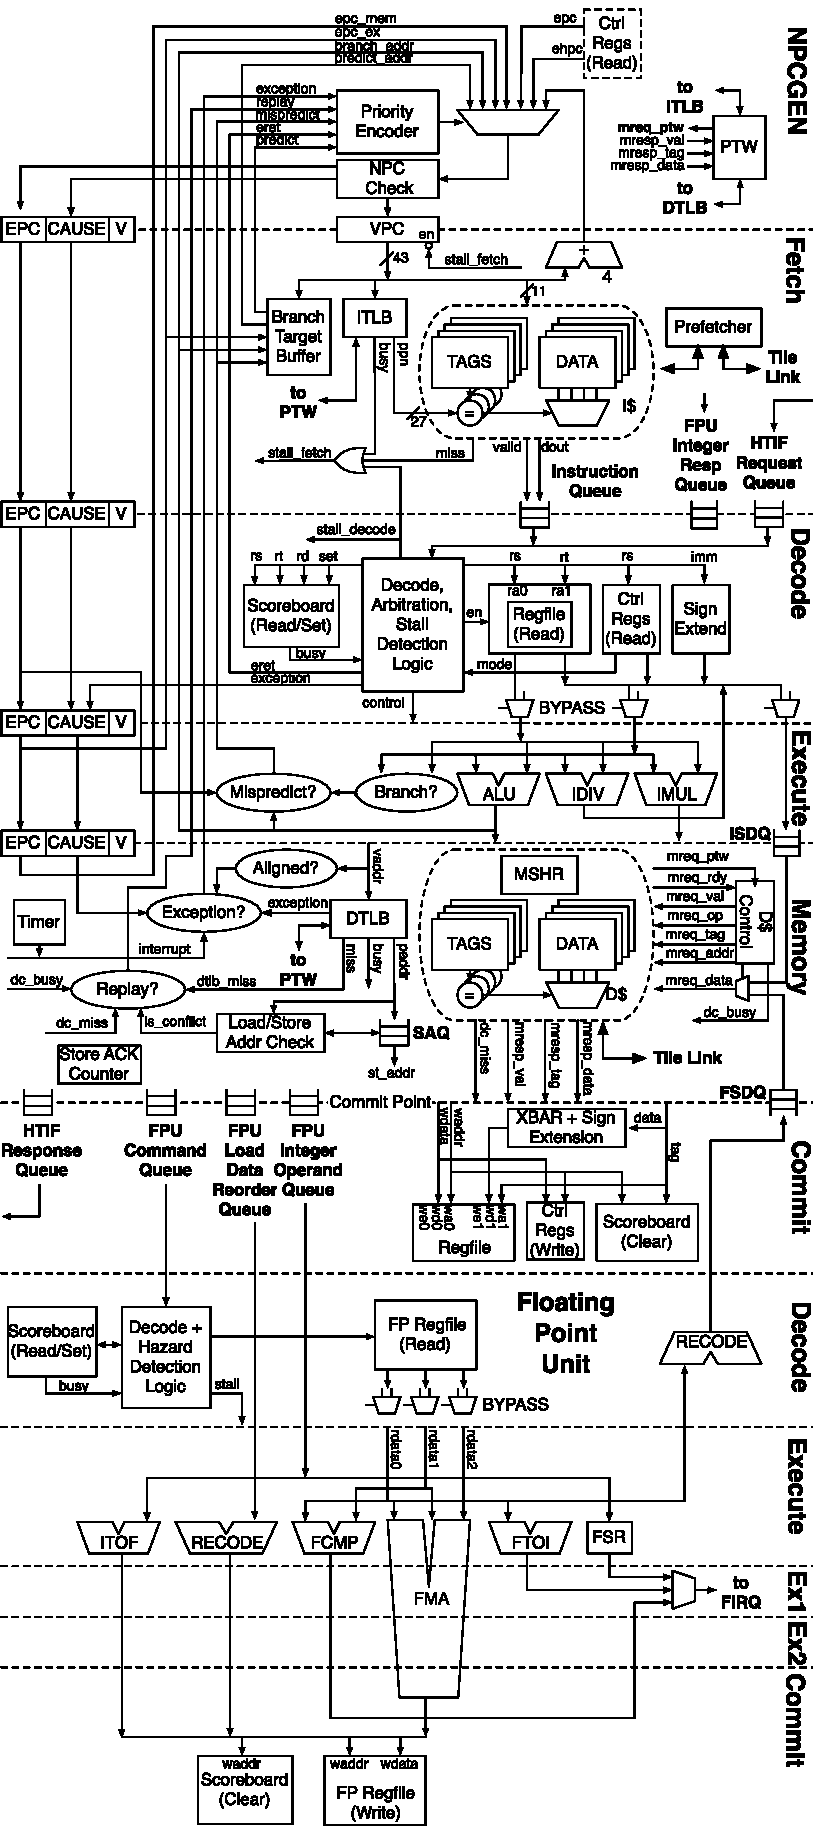
\includegraphics[width=0.65\linewidth]{Images/03_RocketCore_RISCV_Rocket6pipeline.pdf}
    \caption{The Rocket microarchitecture.}
    \label{fig:rocket_core_microarchitecture}
\end{figure}


% Rocket Chip SoC Generator
\subsubsection{Rocket Chip SoC Generator}
Rocket Chip is a highly configurable, open-source System-on-Chip (SoC) generator written in Chisel that produces RISC-V based SoCs \cite{asanovic2016rocketchip}. It is a cornerstone of the Chipyard framework.

% What it is
Instead of being a fixed processor design, Rocket Chip is a generator capable of producing a wide variety of SoC configurations. It can generate systems ranging from simple microcontrollers to complex, multi-core SoCs capable of booting full operating systems.

% Key Components
Key components generated or managed by Rocket Chip include:
\begin{itemize}
    \item \textbf{CPU Cores (e.g., Rocket core):} Generates scalar in-order cores like the Rocket core, or more complex out-of-order cores like BOOM. These cores are highly parameterizable in terms of ISA features, pipeline depth, cache parameters, etc.
    \item \textbf{Cache Hierarchy:} Includes configurable L1 instruction and data caches for each core, and an optional shared L2 cache. Parameters like size, associativity, and replacement policies are customizable.
    \item \textbf{Memory Interconnect (TileLink):} Employs TileLink, an open-source, cache-coherent, chip-scale interconnect protocol designed to connect cores, caches, memory controllers, and peripherals \cite[p.~6]{asanovic2016rocketchip} \cite[p.~15]{chipyard}.
    \item \textbf{Peripheral Interfaces and RoCC Interface:} Provides standard bus interfaces for peripherals and the Rocket Custom Coprocessor (RoCC) interface for integrating custom accelerators.
\end{itemize}

% Why use it
The open-source nature of Rocket Chip, its high degree of configurability via Chisel parameters, and its seamless integration within the Chipyard ecosystem make it an ideal choice for academic research and custom SoC development. It allows for detailed exploration of the design space and rapid prototyping.

\subsection{RISC-V and Rocket Chip Implementation and Relevance to Project}
\label{sec:riscv_rocket_implementation}
% Your Specific Rocket Core Configuration
For this project, a specific configuration of the Rocket core was utilized, instantiated as part of the \texttt{Rocket64b1gem16} SoC. This is a 64-bit (RV64G) Rocket core, configured as a "big" core variant. This implies:
\begin{itemize}
    \item It implements the RV64IMAFD (RV64G) instruction set, including integer, multiplication/division, atomic, single-precision, and double-precision floating-point operations. The `vivado-risc-v` project also suggests the inclusion of the `Zmmul` standard extension for integer multiplication and `Zihintnt` (non-temporal hints) which might be part of the base `gc` configuration used.
    \item It is an in-order, single-issue scalar processor, likely with a 5-stage pipeline as is typical for Rocket cores.
    \item Crucially, it includes a Memory Management Unit (MMU) and supports Supervisor mode, which are essential for running a sophisticated operating system like Debian Linux.
    \item It features configurable branch prediction mechanisms and non-blocking data caches.
\end{itemize}
This Rocket CPU acts as the main general-purpose processor in the SoC, responsible for executing the Linux operating system, managing system resources and peripherals, and dispatching tasks to the Gemmini accelerator.

% Cache Hierarchy
The SoC's memory hierarchy, centered around the Rocket core, includes:
\begin{itemize}
    \item \textbf{L1 Caches:} The Rocket core is equipped with private L1 instruction and data caches. The specific sizes and associativities are parameters set during the Chipyard configuration (e.g., typically 16KB or 32KB, 4-way or 8-way set associative for a "big" core configuration).
    \item \textbf{L2 Cache:} A shared L2 cache is integrated into the system. This cache is inclusive, meaning it maintains a superset of the data stored in the CPU's private L1 caches. The L2 cache serves to reduce average memory access latency for the CPU and can also benefit Gemmini's DMA transfers. The size and associativity of the L2 cache are also configurable parameters (e.g., 512KB or 1MB).
\end{itemize}

% Memory Subsystem
The Rocket core interacts with the rest of the SoC's memory system via the TileLink interconnect. This includes accessing the shared L2 cache and, through it, the main off-chip DDR memory. The MMU within the Rocket core handles virtual-to-physical address translation for memory accesses originating from the CPU. The memory subsystem is designed to be coherent, ensuring a consistent view of memory between the CPU caches and other bus masters like Gemmini's DMA engine.

% Integration within Chipyard
The Rocket Chip parameters for the core (ISA extensions, pipeline features, FPU presence) and the cache hierarchy (L1/L2 sizes, associativity, banking) were specified within the Chipyard SoC configuration files. Chipyard then invoked the Rocket Chip generators to produce the corresponding RTL for these components and integrated them with other parts of the SoC, such as the Gemmini accelerator and the system interconnect.

\section{Gemmini Accelerator as AI Core}
\label{sec:gemmini_ai_core}

\begin{figure}[htbp]
    \centering
    
\includegraphics[width=0.75\linewidth]{Images/04_Gemmini_Logo.pdf}
    \caption{Gemmini logo.}
    \label{fig:gemmini_logo}
\end{figure}

\subsection{Theoretical Aspects of Gemmini}
\label{sec:gemmini_theoretical}
% Need for AI Accelerators
\subsubsection{Need for AI Accelerators}
General-purpose CPUs, while versatile, are often inefficient for the computationally intensive workloads characteristic of modern Artificial Intelligence (AI) and Deep Learning (DL) applications. Operations like matrix multiplication and convolution, which are fundamental to Deep Neural Networks (DNNs), involve massive parallelism that CPUs struggle to exploit effectively. This has driven the development of specialized hardware accelerators designed to perform these tasks with significantly higher performance and energy efficiency.

% Systolic Arrays
\subsubsection{Systolic Arrays}
Systolic arrays are a class of parallel processing architectures particularly well-suited for AI/DL workloads, especially matrix multiplication. They consist of a regular grid of simple Processing Elements (PEs), where data flows rhythmically across the array in a pipelined fashion. Each PE performs a small computation (e.g., a multiply-accumulate operation) and passes its result to neighboring PEs. This architecture allows for high data reuse and parallelism, leading to high throughput and efficiency for structured computations like those found in DNNs \cite{kung1982systolic}.

% What is Gemmini?
\subsubsection{What is Gemmini?}
Gemmini is an open-source, highly configurable systolic array-based matrix multiplication accelerator generator, written in Chisel \cite{genc2019gemmini, chipyard}. It is designed to be integrated into SoCs, often as a Rocket Custom Coprocessor (RoCC) or a TileLink-attached peripheral, to accelerate machine learning inference and training tasks. Gemmini aims to provide a flexible and powerful hardware solution for DNN computations.

\begin{figure}[htbp]
    \centering
    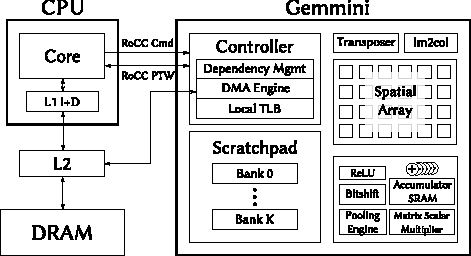
\includegraphics[width=0.75\linewidth]{Images/04_Gemmini_ArchitectureOverview.pdf}
    \caption{Gemmini hardware architectural template overview.}
    \label{fig:gemmini_architecture}
\end{figure}

% Key Architectural Features
\subsubsection{Key Architectural Features of Gemmini}
Gemmini's architecture is defined by several key configurable features:
\begin{itemize}
    \item \textbf{Systolic Array Dimensions (\texttt{DIM}):} The core of Gemmini is a 2D systolic array of PEs. The \texttt{DIM} parameter specifies the size of this array (e.g., a \texttt{DIM} of 16 means a 16x16 array of PEs). The number of PEs directly impacts the parallel processing capability and thus the peak performance of the accelerator.
    \item \textbf{Scratchpad Memory:} Gemmini includes dedicated on-chip SRAM, known as scratchpad memory, for storing input activations (feature maps), weights (filters), and intermediate partial sums. This local memory is crucial for reducing data movement to/from off-chip main memory, thereby saving energy and bandwidth, and enabling high data reuse within the systolic array. Its size is configurable.
    \item \textbf{Accumulator Register File/Memory:} Separate memory or register files are used within or alongside the PEs to accumulate partial sums during matrix multiplication. These accumulators are typically wider than the input data to maintain precision (e.g., 32-bit accumulators for 8-bit input data).
    \item \textbf{Dataflow Strategy:} Gemmini can support different dataflow patterns within its systolic array, such as Output Stationary (OS) or Weight Stationary (WS). In an OS dataflow, output values remain stationary in PEs while inputs and weights are streamed through. In a WS dataflow, weights are pre-loaded and remain stationary in PEs while inputs and outputs move. The choice of dataflow can impact performance and energy efficiency depending on the layer type and dimensions in a neural network. Gemmini is often configured to support both, allowing runtime selection.
    \item \textbf{Custom Instruction Set:} When integrated as a RoCC accelerator, Gemmini is controlled by the host CPU (e.g., Rocket core) through a set of custom RISC-V instructions. These instructions are used to configure Gemmini, load data into its scratchpad, initiate computation, and retrieve results.
    \item \textbf{Data Types and Quantization Support:} Gemmini can be configured to support various data types, with a strong emphasis on quantized integers (e.g., 8-bit integers, INT8) which are widely used in DL inference for efficiency. It includes hardware support for handling scaling factors associated with quantization.
    \item \textbf{DMA Engine:} A Direct Memory Access (DMA) engine is typically part of Gemmini, allowing it to autonomously transfer data between its scratchpad memories and the main system memory (e.g., DDR RAM) over the SoC interconnect (e.g., TileLink).
\end{itemize}

\subsection{Gemmini Implementation and Relevance to Project}
\label{sec:gemmini_implementation}
% Your Specific Gemmini Configuration
In this project, the Gemmini accelerator integrated into the \texttt{Rocket64b1gem16} SoC has the following specific configuration:
\begin{itemize}
    \item \textbf{Systolic Array Dimensions (\texttt{DIM}):} A $16 \times 16$ array of Processing Elements (PEs). This means Gemmini can perform $16 \times 16 = 256$ multiply-accumulate (MAC) operations per clock cycle.
    \item \textbf{Scratchpad Memory:} A 256KB SRAM-based scratchpad memory is provisioned within Gemmini. This memory is used for buffering input activations and model weights. It is typically banked (e.g., 4 banks) to allow for concurrent memory accesses to sustain the data rate required by the PEs.
    \item \textbf{Accumulator Memory:} A separate 64KB memory is dedicated to storing the partial sums and final accumulated values. This memory supports wider data paths for the 32-bit accumulated values and is also banked (e.g., 2 banks).
    \item \textbf{Data Precision:} The accelerator is configured to process 8-bit signed integer input data (INT8) and utilizes 32-bit signed integers for its internal accumulators. This directly supports 8-bit quantized integer arithmetic for DNN inference. Gemmini includes hardware logic for applying quantization scaling factors.
    \item \textbf{Dataflow Versatility:} The Gemmini instance supports both Weight Stationary (WS) and Output Stationary (OS) dataflows, allowing the runtime software or compiler to choose the most efficient strategy for different neural network layers.
    \item \textbf{Ancillary DNN Operations:} The Gemmini unit is configured with hardware support for common DNN operations beyond MACs, such as max pooling and various non-linear activation functions (e.g., ReLU).
    \item \textbf{Local TLB:} Gemmini includes its own 4-entry Translation Lookaside Buffer (TLB) to cache virtual-to-physical address translations for its DMA operations, improving performance in a virtual memory environment.
\end{itemize}

% Integration Method
Gemmini is integrated into the SoC as a Rocket Custom Coprocessor (RoCC) accelerator. This allows the Rocket CPU to issue custom RISC-V instructions to Gemmini for configuration, data movement (via DMA), and computation. The RoCC interface enables Gemmini to interact with the memory system, potentially sharing the CPU's L1 data cache and Page Table Walker (PTW) or connecting directly to the TileLink fabric for higher bandwidth access.

% Data Path
Data is moved between the Rocket core's caches/main memory and Gemmini's scratchpad primarily through Gemmini's dedicated DMA engine. The DMA communicates with the main system memory over a 64-bit wide data bus via the TileLink interconnect. The instructions dispatched by the CPU to Gemmini (e.g., \texttt{mvin} for loading inputs/weights, \texttt{mvout} for storing results) trigger these DMA transfers. These DMA operations are coherent with the CPU caches.

% Rationale for Your Configuration
The $16 \times 16$ systolic array dimensions, 256KB scratchpad, and 8-bit integer support were chosen to provide a balance between significant acceleration for DNN-based time-series anomaly detection models and the available resources on the target FPGA (Xilinx VC707). This configuration is capable of delivering substantial parallel processing for matrix operations common in LSTMs, Transformers, or specialized CNNs used for sequential data. The on-chip memory sizes are intended to hold substantial portions of time-series data segments and model parameters locally, minimizing off-chip memory access. The 8-bit quantization support is crucial for deploying efficient models with reduced memory footprint and bandwidth requirements, aiming for high throughput in anomaly detection tasks while preserving accuracy.

\section{Linux on RISC-V SoCs}
\label{sec:linux_on_riscv}

\subsection{Theoretical Aspects of Linux on RISC-V}
\label{sec:linux_riscv_theoretical}
% Importance of Operating Systems
\subsubsection{Importance of Operating Systems}
Running a full-featured operating system like Linux on custom SoCs, even in embedded contexts, offers significant advantages. These include robust resource management (memory, peripherals), multitasking capabilities, networking stacks, familiar development environments, and access to a vast ecosystem of existing software, libraries, and tools. For complex applications like those involving AI model deployment and data processing, an OS like Linux provides an indispensable foundation.

% Linux Porting for RISC-V
\subsubsection{Linux Porting for RISC-V}
The RISC-V ISA's open nature has spurred significant effort in porting Linux to the architecture. This involves developing a RISC-V architecture-specific port of the Linux kernel, including support for the RISC-V privileged architecture, interrupt handling, and memory management. While the base port is mature, porting Linux to a *new* custom SoC requires ensuring that the SoC hardware (CPU, memory controllers, peripherals) is compatible and that necessary drivers are available or can be developed.

% Boot Process Components
\subsubsection{Boot Process Components}
A typical Linux boot process on an embedded RISC-V SoC involves several key software components:
\begin{itemize}
    \item \textbf{Boot ROM:} The very first code executed on power-on or reset. It performs minimal hardware initialization and typically loads the next stage bootloader from a non-volatile memory source (e.g., SPI flash, SD card).
    \item \textbf{OpenSBI (RISC-V Supervisor Binary Interface):} OpenSBI is an open-source reference implementation of the RISC-V SBI specification. It runs in Machine mode (M-mode) and provides a standardized interface for Supervisor mode (S-mode) software, such as U-Boot or the Linux kernel, to access M-mode functionalities (e.g., console I/O, timer programming, inter-processor interrupts). This abstraction simplifies the porting of S-mode software to different RISC-V platforms \cite{opensbi_project}.
    \item \textbf{U-Boot (Universal Bootloader):} A widely used open-source bootloader for embedded systems. U-Boot performs more extensive hardware initialization (e.g., DDR memory controller, network interfaces), loads the Linux kernel image and Device Tree Blob (DTB) into RAM, sets kernel boot arguments, and then transfers execution to the kernel.
    \item \textbf{Linux Kernel:} The core of the operating system. The RISC-V Linux kernel, once loaded, initializes its own subsystems, probes for hardware devices described in the DTB, mounts the root filesystem, and starts the initial user-space process (e.g., \texttt{init}).
    \item \textbf{Root Filesystem (RFS):} Contains the user-space applications, libraries, configuration files, and system utilities that form the complete Linux distribution (e.g., Debian, Ubuntu, Buildroot, Yocto). It is typically stored on an SD card, eMMC, or network file system.
    \item \textbf{Device Tree Blob (DTB):} A data structure, usually passed by U-Boot to the kernel, that describes the hardware components of the specific SoC and board (e.g., CPU type and count, memory map, peripherals, interrupt controllers). It allows a single kernel binary to boot on different hardware configurations by abstracting hardware details.
\end{itemize}

\subsection{Linux on RISC-V Implementation and Relevance to Project}
\label{sec:linux_riscv_implementation}
% Your Software Stack
The software stack enabling Linux on the custom \texttt{Rocket64b1gem16} SoC, primarily facilitated by the \texttt{vivado-risc-v} project infrastructure, consists of:
\begin{itemize}
    \item \textbf{OpenSBI:} A version compiled as part of the \texttt{vivado-risc-v} build process, specific to its platform definition, often incorporating patches. It acts as the M-mode firmware.
    \item \textbf{U-Boot:} A U-Boot version tailored for the RISC-V SoC environment, using a specific defconfig (e.g., \texttt{vivado\_riscv64\_defconfig}) and patches provided by \texttt{vivado-risc-v}. It is responsible for loading the Linux kernel.
    \item \textbf{Linux Kernel:} A stable Linux kernel version (e.g., from \texttt{linux-stable}), patched and configured by \texttt{vivado-risc-v} to include drivers for FPGA-specific AXI peripherals (like SD card and Ethernet controllers) and other necessary configurations for the custom SoC.
    \item \textbf{Root Filesystem:} A Debian-based RISC-V root filesystem (e.g., \texttt{rootfs.tar.gz} provided or built by \texttt{vivado-risc-v}), deployed on an SD card.
\end{itemize}

% Boot Sequence on Your SoC
The boot sequence on the target FPGA (Xilinx VC707) programmed with the \texttt{Rocket64b1gem16} SoC is as follows:
\begin{enumerate}
    \item \textbf{FPGA Boot ROM:} On power-up, the Rocket core begins execution from a small Boot ROM synthesized into the FPGA. This Boot ROM (contents derived from \texttt{bootrom.img} generated by \texttt{vivado-risc-v} using device tree sources) locates and loads the first stage of the main bootloader (OpenSBI + U-Boot payload, as \texttt{boot.elf}) from the SD card.
    \item \textbf{OpenSBI Initialization:} The loaded \texttt{boot.elf} starts with OpenSBI, which initializes the M-mode environment and prepares for S-mode execution.
    \item \textbf{U-Boot Execution:} OpenSBI transfers control to its payload, U-Boot. U-Boot initializes DDR memory, the SD card controller, and other peripherals. It then loads the Linux kernel image (e.g., \texttt{Image}) and the flattened device tree blob (DTB) from the SD card into DDR memory.
    \item \textbf{Linux Kernel Boot:} U-Boot passes control to the Linux kernel. The kernel initializes itself, uses the DTB to discover and initialize hardware (including the Gemmini accelerator as a RoCC device if described), mounts the Debian root filesystem from the SD card, and starts the user-space environment, eventually providing a Linux login prompt (typically via UART/serial console).
\end{enumerate}

% FPGA Realization
The \texttt{Rocket64b1gem16} SoC RTL, generated by Chipyard, is synthesized and implemented on a Xilinx VC707 FPGA board. This process involves:
\begin{itemize}
    \item \textbf{Synthesis and Place \& Route:} Using the Xilinx Vivado Design Suite (e.g., version 2024.2 as indicated by project context). The \texttt{vivado-risc-v} project provides scripts to automate the creation of a Vivado project, synthesis of the Verilog RTL, implementation (place and route), and generation of the FPGA bitstream (\texttt{.bit} file).
    \item \textbf{Peripheral Integration:} The \texttt{vivado-risc-v} project also supplies Verilog-based peripheral controllers (e.g., for DDR memory via Vivado IP, open-source UART, SD card, and Ethernet controllers) that are integrated with the Chipyard-generated SoC within the Vivado project.
    \item \textbf{Bitstream Loading:} The generated bitstream is loaded onto the VC707 FPGA (e.g., via JTAG using Vivado Hardware Manager or from an on-board flash memory), configuring the FPGA to embody the custom SoC.
\end{itemize}
Successfully booting Debian Linux on the FPGA demonstrates that the custom SoC, including the Rocket core, memory system, Gemmini accelerator interface, and peripherals, are functioning correctly.

% Software Development Environment
Software development for applications running on the Linux environment of the SoC involves:
\begin{itemize}
    \item \textbf{Cross-Compilation Toolchain:} A RISC-V cross-compiler (e.g., GCC provided by Chipyard or \texttt{vivado-risc-v}) running on a host development machine (e.g., x86 Linux PC) is used to compile C/C++ applications for the RISC-V target.
    \item \textbf{Application Deployment:} Compiled applications are transferred to the target system (e.g., via SD card, or over network using SSH/SCP if Ethernet is functional).
    \item \textbf{Execution and Debugging:} Applications are run from the Linux command line on the FPGA. Debugging can be done using GDB with remote debugging capabilities (gdbserver on target, GDB on host), or through serial console print statements. The JTAG interface, supported by \texttt{vivado-risc-v}, can also be used for lower-level hardware debugging.
\end{itemize}
This complete hardware and software environment transforms the FPGA into a functional RISC-V Linux platform, suitable for developing, deploying, and testing the Gemmini-accelerated time-series anomaly detection application.